%=========================================================================
% (c) 2011, 2012 Josef Lusticky

\chapter{Protothreads example}\label{app:protothreads}
Here is
%Next page shows
an example of delaying text on an LCD panel using Protothreads.
It is taken from
Adam Dunkels' Protothreads website~\cite{adam-protothreads} and slightly modified.
Protothreads can be used for introducing delays inside a function, without using a full threading model.
The example shows a function writing characters to LCD panel.
Suppose each character is shown for one second, then next character replaces previous.
\begin{lstlisting}[numbers=left]
#include "pt.h"
#include "timer.h"
#include <string.h>

typedef unsigned short lc_t;

struct pt {
  lc_t lc;                                           /* Local continuation */
};

struct pt state;
struct timer timer;

PT_THREAD(display_text(struct pt *pt, const char *msg))
{
  PT_BEGIN(pt);
  for (int i = 0; i < strlen(msg); i++) {
    lcd_display_char(msg[i]);
    timer_set(&timer, CLOCK_SECOND);               /* Wait for one second. */
    PT_WAIT_UNTIL(pt, timer_expired(&timer));
  }
  PT_END(pt);
}

int main(void)
{
  PT_INIT(&state);
  for (;;) {
    display_text(&state, "Hello world");
    /* Here can be another thread run */
  }
  return 0;
}
\end{lstlisting}
%\newpage
The PT\_WAIT\_UNTIL macro actually causes the function to return.
While the function is waiting for the timer to expire another function can be called and run.
When the function is entered again the execution continues with the PT\_WAIT\_UNTIL macro
which causes the function to check the condition it is waiting for (timer expired).
If the condition is met the function resumes, if not it returns again.
Strictly speaking the amount of time between showing each character can
be more than one second.
This is because Protothreads are not running simultaneously: when the timer expires
and another Protothread is running, this Protothread would have to wait until
it is entered again. Than the condition specified in PT\_WAIT\_UNTIL is met and
next iteration of loop started, that is, next character is displayed.

How does it work? The macro PT\_BEGIN is expanded to {\it switch} statement while preprocessing the
code for compilation.
The PT\_WAIT\_UNTIL macro expands to {\it case} and setting the local continuation
to the value, so that next time this function is run, it jumps to this {\it case}.
The structure holding the state is defined outside of the function so its context is not lost when
the function returns. The simplest state structure would hold just the local continuation variable.

Now follows
%Next page shows
the same sample of code after simplified preprocessing.
%\newpage
\begin{lstlisting}[numbers=left]
#include "pt.h"
#include "timer.h"
#include <string.h>

typedef unsigned short lc_t;

struct pt {
  lc_t lc;                                           /* Local continuation */
};

struct pt state;
struct timer timer;

int display_text(struct pt *pt, const char *msg)     /* Expanded PT_THREAD */
{
  switch(pt->lc) {  case 0:                      /* Expanded PT_BEGIN(pt); */

    for (int i = 0; i < strlen(msg); i++) {
      lcd_display_char(msg[i]);
      timer_set(&timer, CLOCK_SECOND);             /* Wait for one second. */

                                   /* The following two lines are expanded */
      pt->lc = 31; case 31:   /* PT_WAIT_UNTIL(pt, timer_expired(&timer)); */
      if(!(timer_expired(&timer))) { return PT_WAITING; }         /* macro */

    }

  pt->lc = 0; return PT_ENDED; }                        /* Expanded PT_END */

}

int main(void)
{
  state->lc = 0;                                       /* Expanded PT_INIT */
  for (;;) {
    display_text(&state, "Hello world");
    /* Here can be another thread run */
  }
  return 0;
}

\end{lstlisting}

\chapter{Clock interrupt frequency measurements}\label{app:interrupt-frequency}
\begin{figure}[h!]
  \centering
  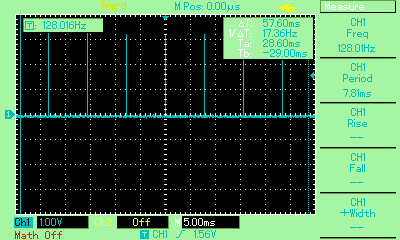
\includegraphics[width=10cm,keepaspectratio]{fig/osc-no-adjust.png}
  \caption{Interrupt frequency without clock adjustment}
  \label{fig:osc-no-adjust}
  \bigskip
\end{figure}

\begin{figure}[h!]
  \centering
  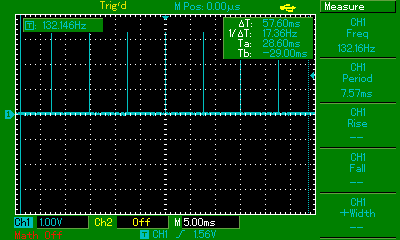
\includegraphics[width=10cm,keepaspectratio]{fig/osc-speed-up.png}
  \caption{Interrupt frequency when speeding up the clock}
  \label{fig:osc-speed-up}
  \bigskip
\end{figure}

\begin{figure}[h!]
  \centering
  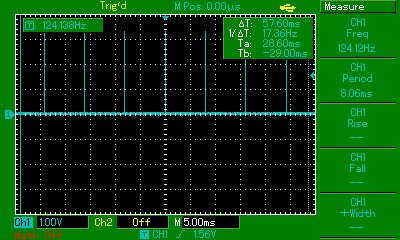
\includegraphics[width=10cm,keepaspectratio]{fig/osc-slow-down.png}
  \caption{Interrupt frequency when slowing down the clock}
  \label{fig:osc-slow-down}
  \bigskip
\end{figure}


\chapter{Clock phase difference measurements}\label{app:phase}
The following figures show the output from UNI-T~2025CEL digital oscilloscope.
The yellow line on~channel~2 shows the impulses from the GPS synchronised clock Meinberg~GPS~167.
The blue line on~channel~1 shows the impulses from AVR Raven running
Contiki~OS with the developed NTP client.
The rising edge occurs when each second is being accounted.
\begin{figure}[h!]
  \centering
  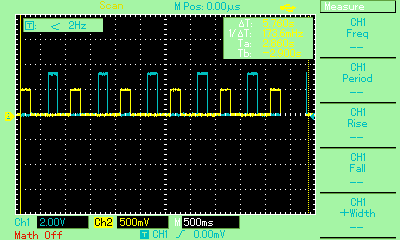
\includegraphics[width=10cm,keepaspectratio]{fig/osc-out-of-phase.png}
  \caption{Second impulses when the clock is out of phase}
  \label{fig:osc-out-of-phase}
  \bigskip
\end{figure}

\begin{figure}[h!]
  \centering
  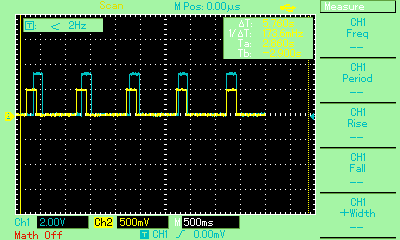
\includegraphics[width=10cm,keepaspectratio]{fig/osc-adjusting-phase.png}
  \caption{Second impulses when the clock is being adjusted}
  \label{fig:osc-adjusting-phase}
  \bigskip
\end{figure}

\begin{figure}[h!]
  \centering
  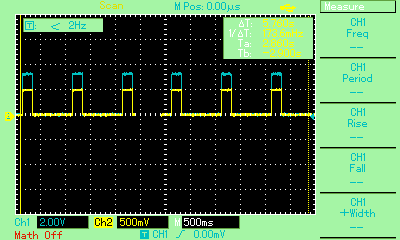
\includegraphics[width=10cm,keepaspectratio]{fig/osc-in-phase.png}
  \caption{Second impulses when the clock is in phase}
  \label{fig:osc-in-phase}
  \bigskip
\end{figure}


\chapter{CD Content} %!TODO
\begin{tabular}{|l|l|}
	\hline
	Directory & Content \\ \hline
	docs/ & Setup guides for running and debugging Contiki OS on AVR Raven\\
	docs/datasheets/ & Datasheets for used hardware\\
	docs/img/ & Images from Dopsy group laboratory at RheinMain University\\
	sw/ntpd/ & Contiki NTP Client source code\\
	sw/test/ & Program used for testing Contiki NTP Client\\
	\hline
\end{tabular}
